\section{Overview}
\label{sec:intro}

Secure remote computation (Figure~\ref{fig:remote_computation}) is the problem
of executing software on a remote computer \textbf{owned and maintained by an
untrusted party}, with some integrity and privacy guarantees. In the general
setting, secure remote computation is an unsolved problem. Fully Homomorphic
Encryption \cite{gentry2009fhe} solves the problem for a limited family of
computations, but has an impractical performance overhead
\cite{naehrig2011can}.

\begin{figure}[hbt]
  \centering
  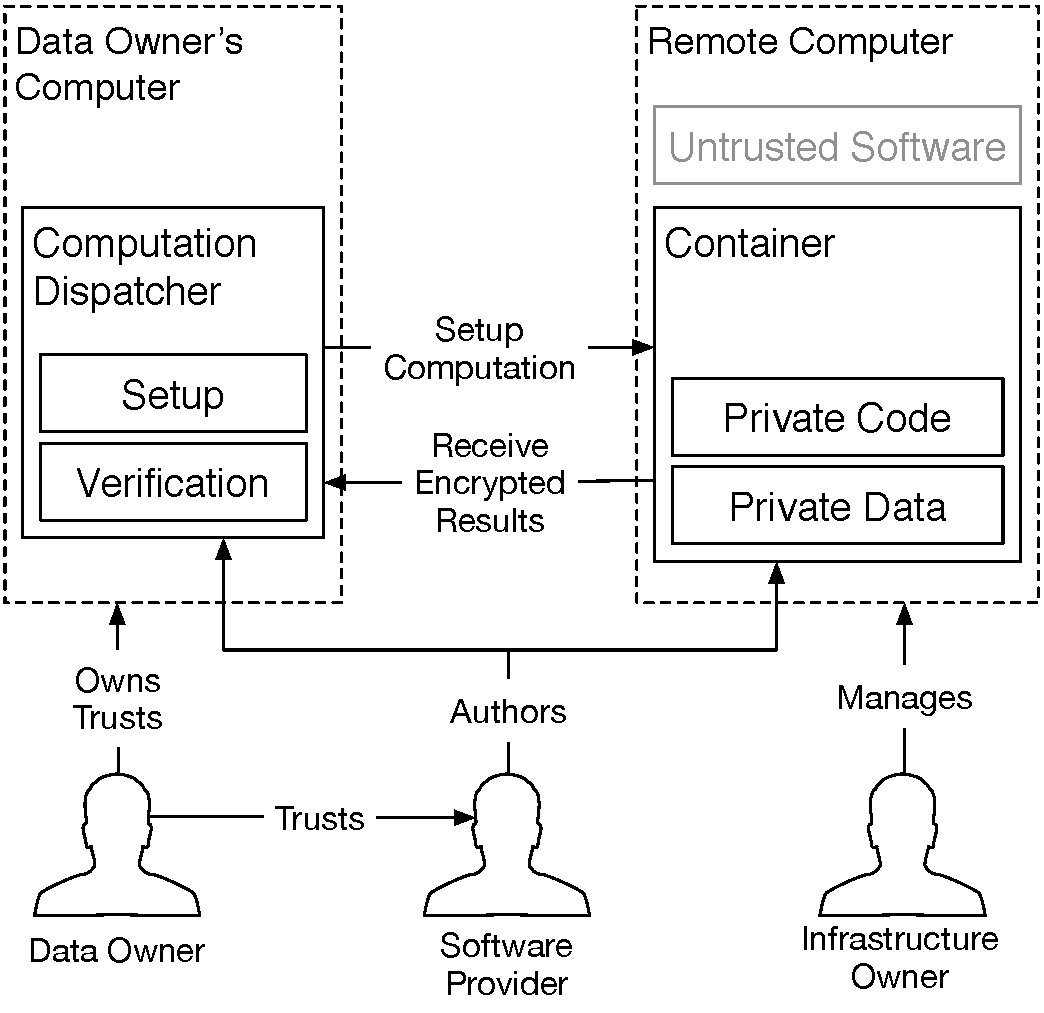
\includegraphics[width=75mm]{figures/remote_computation.pdf}
  \caption{
    Secure remote computation. A user relies on a remote computer, owned by an
    untrusted party, to perform some computation on her data. The user has some
    assurance of the computation's integrity and privacy.
  }
  \label{fig:remote_computation}
\end{figure}

Intel's Software Guard Extensions (SGX) is the latest iteration in a long line
of trusted computing (Figure~\ref{fig:trusted_computing}) designs, which aim to
solve the secure remote computation problem by leveraging trusted hardware in
the remote computer. The trusted hardware establishes a secure container, and
the remote computation service user uploads the desired computation and data
into the secure container. The trusted hardware protects the data's privacy
and integrity while the computation is being performed on it.

\begin{figure}[hbt]
  \centering
  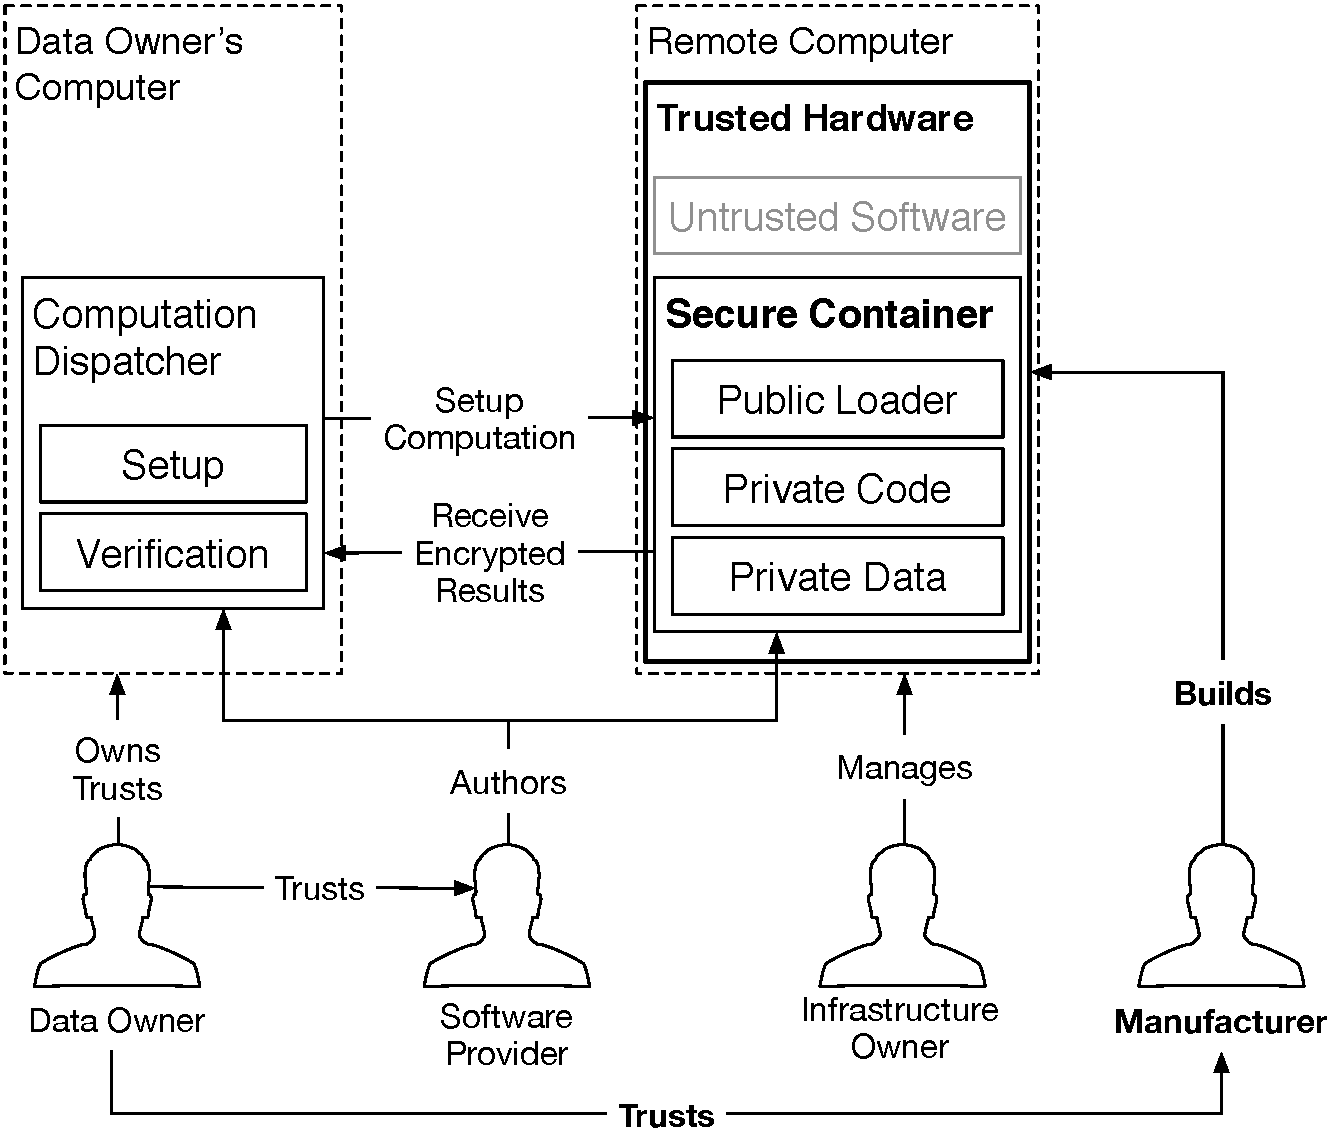
\includegraphics[width=85mm]{figures/trusted_computing.pdf}
  \caption{
    Trusted computing. The user trusts the manufacturer of a piece of hardware
    in the remote computer, and entrusts her data to a secure container hosted
    by the secure hardware.
  }
  \label{fig:trusted_computing}
\end{figure}

SGX relies on \textit{software attestation}, like its predecessors, the
TPM~\cite{grawrock2003tpm} and TXT~\cite{grawrock2009txt}. Attestation
(Figure~\ref{fig:generic_attestation}) proves to a user that she is
communicating with a specific piece of software running in a secure container
hosted by the trusted hardware. The proof is a cryptographic signature that
certifies the hash of the secure container's contents. It follows that the
remote computer's owner can load any software in a secure container, but the
remote computation service user will refuse to load her data into a secure
container whose contents' hash does not match the expected value.

\begin{figure}[hbt]
  \centering
  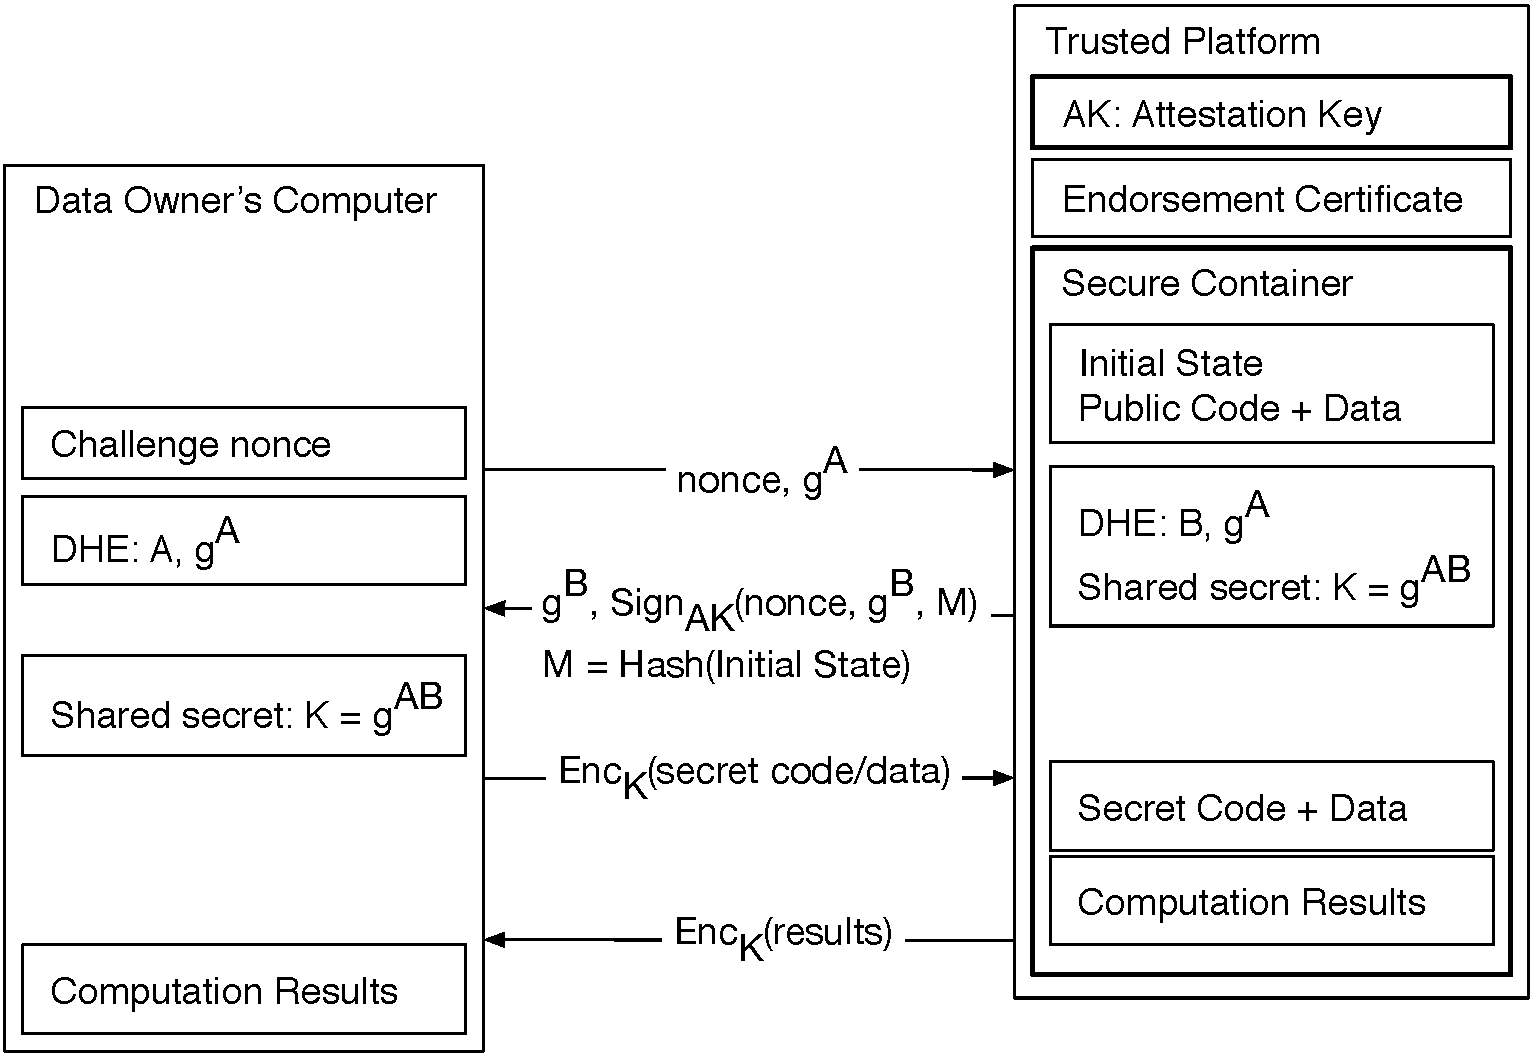
\includegraphics[width=87mm]{figures/generic_attestation.pdf}
  \caption{
    Software attestation proves to a remote computer that it is communicating
    with a specific secure container hosted by a trusted platform. The proof is
    an attestation signature produced by the platform's secret attestation key.
    The signature covers the container's initial state, a challenge nonce
    produced by the remote computer, and a message produced by the container.
  }
  \label{fig:generic_attestation}
\end{figure}

The remote computation service user verifies the \textit{attestation key} used
to produce the signature against an \textit{endorsement certificate} created by
the trusted hardware's manufacturer. The certificate states that the
attestation key is only known to the trusted hardware, and only used for the
purpose of attestation.

SGX stands out from its predecessors by the amount of code covered by the
attestation, which is in the Trusted Computing Base (TCB) for the system using
hardware protection. The attestations produced by the original TPM design
covered all the software running on a computer, and TXT attestations covered
the code inside a VMX \cite{uhlig2005vmx} virtual machine. In SGX, an
\textit{enclave} (secure container) only contains the private data in a
computation, and the code that operates on it.

For example, a cloud service that performs image processing on confidential
medical images could be implemented by having users upload encrypted images.
The users would send the encryption keys to software running inside an enclave.
The enclave would contain the code for decrypting images, the image processing
algorithm, and the code for encrypting the results. The code that receives the
uploaded encrypted images and stores them would be left outside the enclave.

An SGX-enabled processor protects the integrity and privacy of the computation
inside an enclave by isolating the enclave's code and data from the outside
environment, including the operating system and hypervisor, and hardware
devices attached to the system bus. At the same time, the SGX model remains
compatible with the traditional software layering in the Intel architecture,
where the OS kernel and hypervisor manage the computer's resources.

This work discusses the original version of SGX, also referred to as SGX 1.
While SGX 2 brings very useful improvements for enclave authors, it is a small
incremental improvement, from a design and implementation standpoint. After
understanding the principles behind SGX 1 and its security properties, the
reader should be well equipped to face Intel's reference documentation and
learn about the changes brought by SGX 2.


\subsection{SGX Lightning Tour}
\label{sec:intro_sgx}

SGX sets aside a memory region, called the \textit{Processor Reserved Memory}
(PRM, \S~\ref{sec:sgx_prm}). The CPU protects the PRM from all non-enclave
memory accesses, including kernel, hypervisor and SMM (\S~\ref{sec:rings})
accesses, and DMA accesses (\S~\ref{sec:motherboard}) from peripherals.

The PRM holds the \textit{Enclave Page Cache} (EPC, \S~\ref{sec:sgx_epc}),
which consists of 4~KB pages that store enclave code and data. The system
software, which is untrusted, is in charge of assigning EPC pages to enclaves.
The CPU tracks each EPC page's state in the \textit{Enclave Page Cache
Metadata} (EPCM, \S~\ref{sec:sgx_epcm}), to ensure that each EPC page belongs
to exactly one enclave.

The initial code and data in an enclave is loaded by untrusted system software.
During the loading stage (\S~\ref{sec:sgx_enclave_lifecycle}), the system
software asks the CPU to copy data from unprotected memory (outside PRM) into
EPC pages, and assigns the pages to the enclave being setup
(\S~\ref{sec:sgx_epcm}). It follows that the initial enclave state is known to
the system software.

After all the enclave's pages are loaded into EPC, the system software asks the
CPU to mark the enclave as initialized (\S~\ref{sec:sgx_enclave_lifecycle}), at
which point application software can run the code inside the enclave. After an
enclave is initialized, the loading method described above is disabled.

While an enclave is loaded, its contents is cryptographically hashed by the
CPU. When the enclave is initialized, the hash is finalized, and becomes the
enclave's \textit{measurement hash} (\S~\ref{sec:sgx_measurement}).

A remote party can undergo a \textit{software attestation} process
(\S~\ref{sec:sgx_attestation}) to convince itself that it is communicating with
an enclave that has a specific measurement hash, and is running in a secure
environment.

Execution flow can only enter an enclave via special CPU instructions
(\S~\ref{sec:sgx_threads}), which are similar to the mechanism for switching
from user mode to kernel mode. Enclave execution always happens in protected
mode, at ring 3, and uses the address translation set up by the OS kernel and
hypervisor.

To avoid leaking private data, a CPU that is executing enclave code does not
directly service an interrupt, fault (e.g., a page fault) or VM exit. Instead,
the CPU first performs an Asynchronous Enclave Exit (\S~\ref{sec:sgx_aex}) to
switch from enclave code to ring 3 code, and then services the interrupt,
fault, or VM exit.  The CPU performs an AEX by saving the CPU state into a
predefined area inside the enclave and transfers control to a pre-specified
instruction outside the enclave, replacing CPU registers with synthetic values.

The allocation of EPC pages to enclaves is delegated to the OS kernel (or
hypervisor). The OS communicates its allocation decisions to the SGX
implementation via special ring 0 CPU instructions
(\S~\ref{sec:sgx_enclave_lifecycle}). The OS can also evict EPC pages into
untrusted DRAM and later load them back, using dedicated CPU instructions. SGX
uses cryptographic protections to assure the privacy, integrity and freshness
of the evicted EPC pages while they are stored in untrusted memory.
